%!TEX root=thesis.tex
\chapter{Implementation}

% Command - B = compile

\section{Front-End}

We have opted for a minimalistic, simple design for our beta version, as a strategy to iteratively develop it while testing its usability with end-users. This approach facilitates later integration of graphics. The trademarks of our front-end user interface design are: responsiveness, minimalist and intuitive, kids-friendly.\\

\subsection{UI Framework} 
The front-end framework we use is Bootstrap Twitter ( Version XXX ). We have settled on Boostrap after a pros and cons analysis of the alternative frameworks. Although frameworks like Foundation, Semantic UI, Material Design, Ulkit have some competitive features, Boostrap won by having some unbeatable advantages.
It corresponds to one of our core design principles: responsiveness. It exceeds other frameworks by its stated attention towards resposiveness and mobile-friendliness.
Bootstrap is still regarded as the most popular front-end framework, with large community support and consequenlty with rich documentation and resources: articles and tutorials, third-party plug-ins and extensions, theme builders.\\

I prefer Boostrap beacause of its level of specificity. Being more generic than other frameworks that tend to have higher-level specificity, its minimal style framework is easier to customise. I consider it is more practical to add up styling rules than overwriting existing ones. 
(Ref: https://www.sitepoint.com/5-most-popular-frontend-frameworks-compared/)\\

A good framework needs to level up constantly with the latest web technologies, especially with regards to mobile. Bootsrap does that, being constantly under active development. It also has a generous browser support.\\	

Some of the other frameworks have some very competitive features. Semantic UI has some extra unique UI components and outperforms Boostrap as a very friendly, semantic language. Its overall structure of the framework and the naming conventions, in terms of clear logic and semantics of its classes has a clear vantage point. It prounds itself with a scalable and modular architecture for css as main property.
Frameworks such as Semantic UI and Foundation also outweight others by a unique, rich pallette of UI components.
YOOtheme distinguishes itself with a better GUI Customizer. It offers a flexible and powerful customization mechanism, either manually or via its GUI customizer.
Regarding the spectrum of browser support, Boostrap is not the top, being a step behind Foundation.\\

\subsection{Programming Languages and Layout Principles} 
Using mainly Javascript/Jquery => keeping the mark-up language separated from javascript as much as possible. Small modules of javascript code, each javascript file corresponding to an UI component.

Use preprocessor progamming language SCSS, to facilitate a better UI standardization and omogenity. 

A folder dedicated to layout => comprises the main layout elements that are common to all or some of the application pages. 



\section{Back-End}

\subsection{Working Environment Settings} 

Server host provider Meebox, comes with Mysql version XXX as well as it comes with phpMyAdmin installed for database management.

Production + Testing Dbs
Communication Management Tools: Github, Slack.


\subsection{Server-side language} 

I have built the application using the scripting language PHP as server-side choice. I believe it is a reliable choice, as PHP has been steadily one of the most widely used developing language for web applications. It is commonly known for its portability and it is supported by the highest number of web server hosting providers. 
PHP is widely backed by large programming communities and it is open source, which assures a solid development environment, with a steady community commitment in stabilizing it.\\ 

PHP is also known for its flexibility/resilience. It it portable on all major operating systems, can function both as a module or a CGI processor and has support on a wide range of web servers. PHP  holds up both procedural and object-oriented (OOP) programming paradigms, and has compatibility with a collection of databases.\\ 

For relational database management system (RDMS) I have opted for MySql. PHP can use mainstream MySQLLi and provides an abstraction layer through PDO, which I have made use of.

\subsection{RDMS} 

PDO stands for PHP Data Objects. It provides a data-access abstraction layer, using a unified API, which is a lean, consistent way to access databases regardless of the database. This increases the portability of our code, if we want to change the database we operate with.\\

One core advantage of PDO over MySQLi lyes in its database driver support. PDO upholds around 12 different drivers, opposed to MySQLi, which supports MySQL only. This fact has implications for further software changes, as using PDO makes it facile to transfer to a different database.\\  

The abstraction layer PHP offers in interaction with the database through PDO optimises the program execution and maximises security measurements.
The performance is boosted by the use of Prepared Statements, which allows the parsing and execution of a query only once. The queries are sent only once to the database, where they wait for the parameters. The bandwidth to the server is minimalized through the use of Binding Parameters, which are sent independently to the query waiting on the db.\\ 

The second advantage of employing PDO is the layer of security it provides. It is designed to shield against one of the most invasive forms of security breaches: SQL injections. The parameters sent in the query are transmitted later than the query commands using a different protocol. They are scrunitized with security filters through these protocols.\\ 

In the design of our database, we have used all types of relational raports between tables. One-to-one relationship model is predominent, followed by one-to-many pattern. 
The many-to-many relationship is used in merging data between tables such Members-Projects, Projects-Steps, Members-Achievements, Members-Activities, Members-Quizzes, Members-Comments.
I describe the database design using the following Entity Relation Diagram. I have used a coloristic relation map to differentiate the types of dependency between tables and data.
[Sceenshot DB Entity-Relation]\\

\begin{figure}
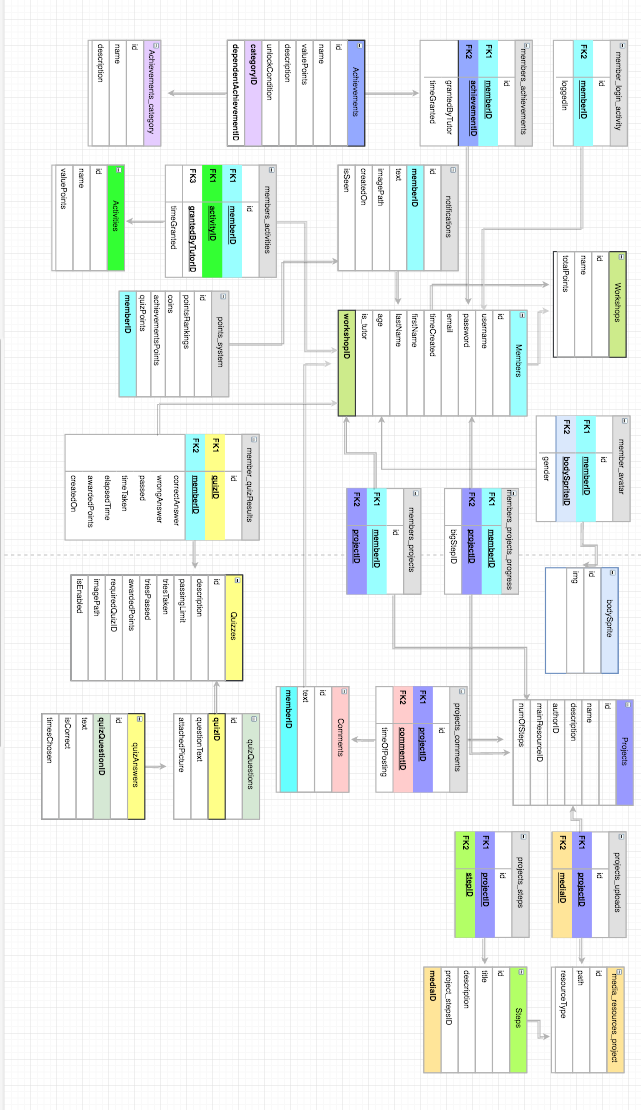
\includegraphics[width=0.8\linewidth]{images/DBEntityRelation.png}
\caption{Database Entity Relation.}
\label{fig:boat1}
\end{figure}


\subsection{Application Architecture and Design Principles}

I have designed my code around few pillarstone principles: separation of concerns, DRY (Do Not Repeat Yourself) and modularity (reusable components). Separation of concern principle is commonly associated with the MVC architecture design pattern. Although I do not employ a standard MVC framework, I have structured the composition of the code by applying MVC patterns, by striving to preserve a neat separation between the business logic and the view.\\ 

I will exemplify the application arhitecture design through the following diagram which describes interactions of the Projects section. 
[Screenshot/Diagram]\\

On Client-side I have separated the plain presentation from functionality, by keeping the the mark-up language from javascript in separate files / I have dissociated the markup language from the javascript, by creating dedicated javascript files. For readability purposes, I structured the front-end code in smaller separate files, so any major ui component is represented by a distinct file. 

Because I make frequent use of Ajax calls, I have decided to dedicate a separate file where I have modelled an ajax API, that defines all ajax calls functions used throughout Projects (ajaxProjectsAPI.js). Doing so, I gain readibility of the code, by having a javascript file that only deals with the actual ajax calls, and the other javascript file only displaying the data in the view. The next advantage I get is modularity. Having a common/universal ajax API for the Projects module, I centralize all the ajax calls under reusable functions, that are accessible from any file of the module and even to other modules. This way, I can use same ajax function when needed and forestall redundancy of code.
For example,(as shown in the diagram) the ajaxUploadFile function is called from different js files of the same module/folder, or can be called from other modules, anywhere in the system.(or change example)\\ 

I'll describe the design of the AJAX API. It has 2 central generalized Ajax calls functions: postAjaxCall and postAjaxCallSendDictParams. postAjaxCall function sends only one parameter as data, while the other takes a dictionary for sending a couple of arguments to the server.
Both functions take the following arguments: the server-side page they are sending data to, the data to be sent (name of the action and parameters), and a function that will be executed (in javascript) if the ajax call has been successful.\\ 

All the other functions of the Ajax API are calling one of the 2 generalized functions, depending on the amount of data they send. 
I have payed attention at functions naming conventions, as part of my clean code effort strategy. Consequently, these functions are suggestively named by the type of action they perform on the back-end, same as the action parameter sent as data.\\

The Ajax API brings me back at the MVC structure pattern, corresponding in a way to the Controller of the MVC design pattern / The Ajax API is for my application what the Controller is for the MVC pattern. It acts as an intermediary between the server-side(business logic) and the front-end(view). Basically, it solicits data from the server and takes the resulted data transffering it to the view, without processing it in any way.\\  

Having the Ajax calls isolated, the other javascript files are left to perform the display of data. I encapsulate the display mechanism in functions as well. 
I have created distinctive functions for each display demand of data in the interface. By doing so, display functions can be reused by other functions and the readibility of the code is increased. Moreover, it increases modularity and it facilitates easy future changes or integration of new components in the UI.
Commonly, a javascript function in the system will call one or more ajax functions and will pass it as argument a display function.\\ 

\begin{figure}
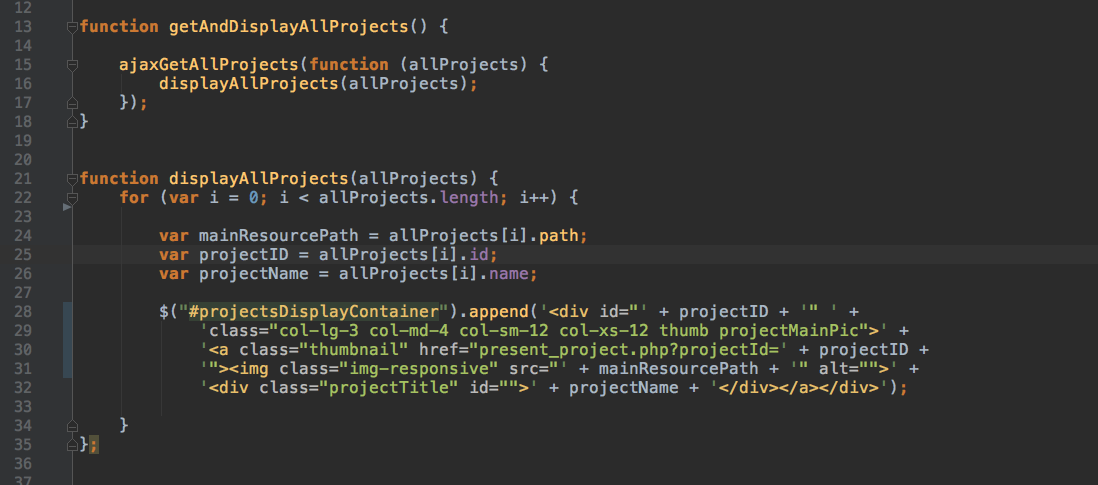
\includegraphics[width=1\linewidth]{images/JavascriptFunction.png}
\caption{Javascript Standard Function.}
\label{fig:javascript_function}
\end{figure}


On Back-end, i organised the API in 2 main files: projects\_functions.php and projects\_server.php. In projects\_server.php are all functions and the database requests/queries called through the Ajax API that are sent to the Data Server, while in projects\_functions all the other functions, associated with the Web Server requests.
Besides the two, I separate the back-end functions for self-supprting actions in independent files, like uploading media resources in upload.php, adding the steps for the project and uploading steps in upload\_steps.

Another code clean priciple I have developed on the way is trying to perform as much calculations/processing of data as possible on the back-end and in queries, obtaining as clear-cut/definite data as needed in front-end (with less functionalities on the javascript). 

\begin{figure}
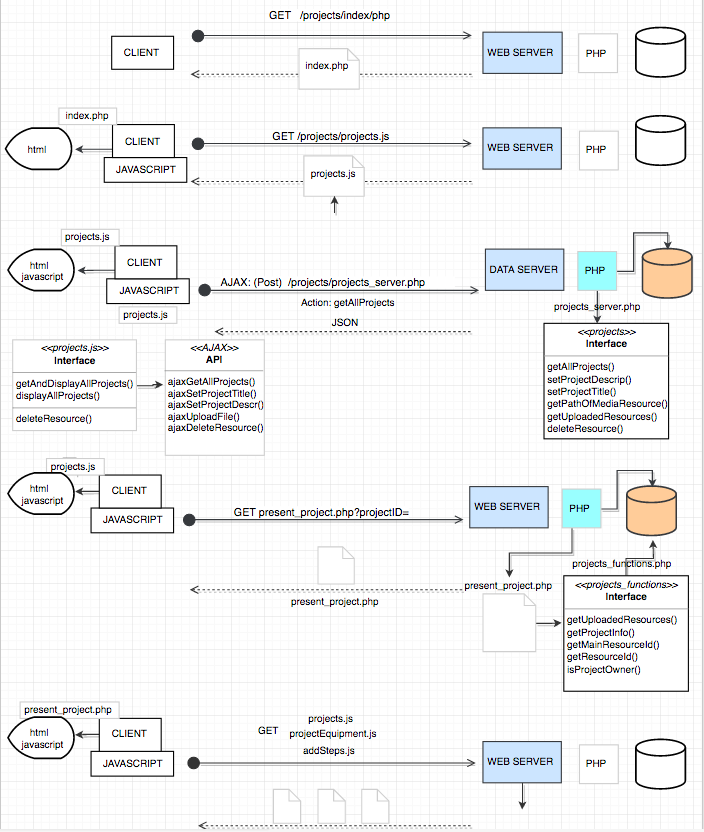
\includegraphics[width=0.8\linewidth]{images/ProjectsArchitecture.png}
\caption{Projects Architecture.}
\label{fig:projects_architecture.}
\end{figure}

[Diagram of interactions between files]


\subsection{Routing and Endpoints}

I combine the use of both a Web Server and a Data Server throughout the application, depending on the amount of data needed and the probability of future reuse of inquired data from the server. I will illustrate the use of both by showcasing the endpoints in /projects. 

Mostly all requests to the server API is done through the POST to one of the endpointsdescribed below. Endpoints which require a user to be authenticated expect a valid session ID in the GET parameter session. Some endpoints allow or require some fields to be submitted
as POST fields, those are expected to be included in the message body as a
application/x-www-form-urlencoded string.

I illustrate the architecture of the system for the /projects/index.php and projects/create\_project.php in the UML diagram below.


\subsection{Show All Projects}
/projects/index.php

This endpoint returns the main page of the projects module, which displays all the existent projects, that can be individually accessed from this page for details. 
The page has a filter by label tags system, through which users can select projects by categories from a given collection of labels. 

I use Ajax for retrieving and displaying the projects that result in the search by labels. I have prefered to dynamically update the page with the selected projects rather than refresh the page, as it was more facile to hide the unselected projects in javascript than updating the page with the previously selected labels. This way, after the Filter on click event is triggered, only the projects section is dynamically changed, the selected labels remaining unchanged.

The page also offers the user the possibility of adding a new project. The 'Add New Project' button will redirect the user to the following url: projects/edit\_project.php?{projectId}. In the background, the redirect actually goes first through  projects/create\_project.php, which sets the ground for the editing phase. I will explain what happens in the following endpoint description.


\subsection{Create New Project}
projects/create\_project.php

This endpoint has only a mediating and rerouting function between /index.php and edit\_project.php, as we need to extract the id of the newly created project in order to save the information while editing the project. For that reason, create\_project.php inserts a new project in the database that has only an id and no other data. Then it extracts the latest inserted id, sending it as an argument to the edit\_project.php?{projectID} and redirecting to the editing page.
[Screenshot] Header("Location: /smartfun/pages/projects/edit\_project.php?projectId=lastInsertedProjectID")

In the end, creating a new project and editing an existing one, both happen in the edit page, as we'll subsequently see.

\subsection{Edit Project}
/projects/edit\_project.php/{projectID}

This endpoint is accessed in two situations. One instance is when the user creates a new project, case in which it receives the id of the new project through a GET protocol from the create\_project.php. The other is when the project was already created and the user only expects to edit the information. This case is accessed from the present\_project page, through an event which is visible only the the admins of the system.

\begin{figure}
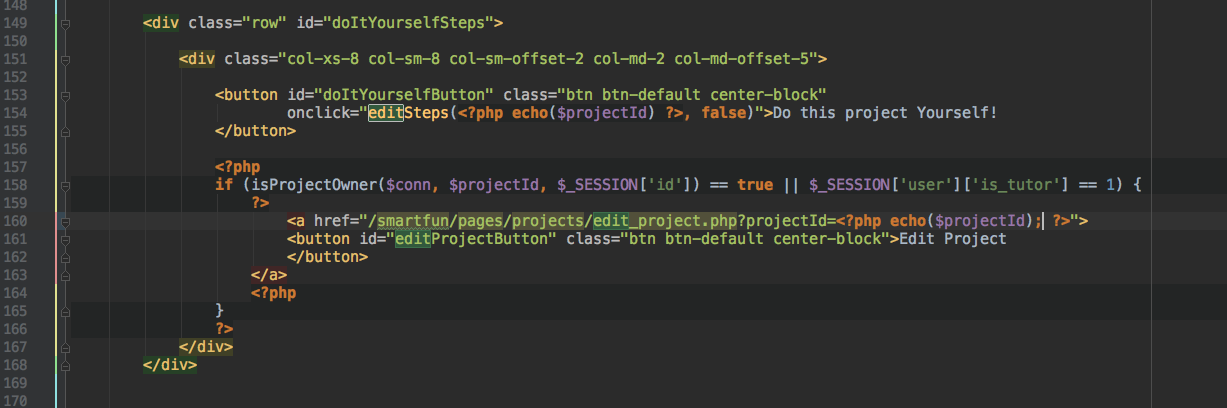
\includegraphics[width=1\linewidth]{images/edit.png}
\caption{Edit Project.}
\label{fig:edit_project.}
\end{figure}	

In any case, the endpoint returns from the web server the existing information about that particular project: title, description, uploaded media resouces, materials list. These are obtained through the API defined in projects\_functions.php, which includes all the requests to the web server.	

All the edited information of the project are sent to the server through the Ajax API. The ajax functions are called by triggered events defined in the projects.js file. 

It also includes projects\_equipment.js and addSteps.js. Adding steps is a core feature of the projects, as each project is presented as a succession of steps. Editing steps means choosing a media resource and description for each individual step. This happens in the same page (on a full-page popup), keeping the mark up and changing dynamically only the content of each step (?!).

 \subsection{Present Project}
/projects/present\_project.php/{projectID}

Gets information from web server about the requested project.
Besides the project description and a carrousel with project pictures, it includes a few dynamic components the user can interact with. present\_project.php include a number of javascipt files, each correspondent to one of these UI components.
One component is the stars rating system, where users can evaluate the project by voting on a 5 stars scale on criterias describing levels of: difficulty, fun and general. In stars\_ratings.js I describe the functions  that show interactions with the ratings system. Each criteria voted in the system is indiviually updated in the database through a concurrent Ajax.

Second dynamic component is projects labels section, where users can participate in adding descriptive tags about the project. In the current version, users can add up any labels that are yet non-existant. We have two alternative scenarios for dealing with the obvious problems this approach raises. We could first pass the labels through an admins filter, or we could leave the feature only for admin use. 

The project equiments section is the third component users can interact with. This component lists all the needed equipments for carrying out the project. Users can check the items they already possess or can send to basket items they would need and like to buy. The events handling for the equipments is encapsulated in projects\_equipment.js. 

Users can exchange ideas through the Comments Section, which can monitored/managed (edited/deleted)by admins.
comments.js processes the events linked to users comments.

The detailed description of how to do the project is contained in the Steps. Steps are the tutorial users are following in order to build the project. We use the same UI component for displaying the steps as for editing them, by using control structures and javascript hide and display functions. 

\begin{figure}
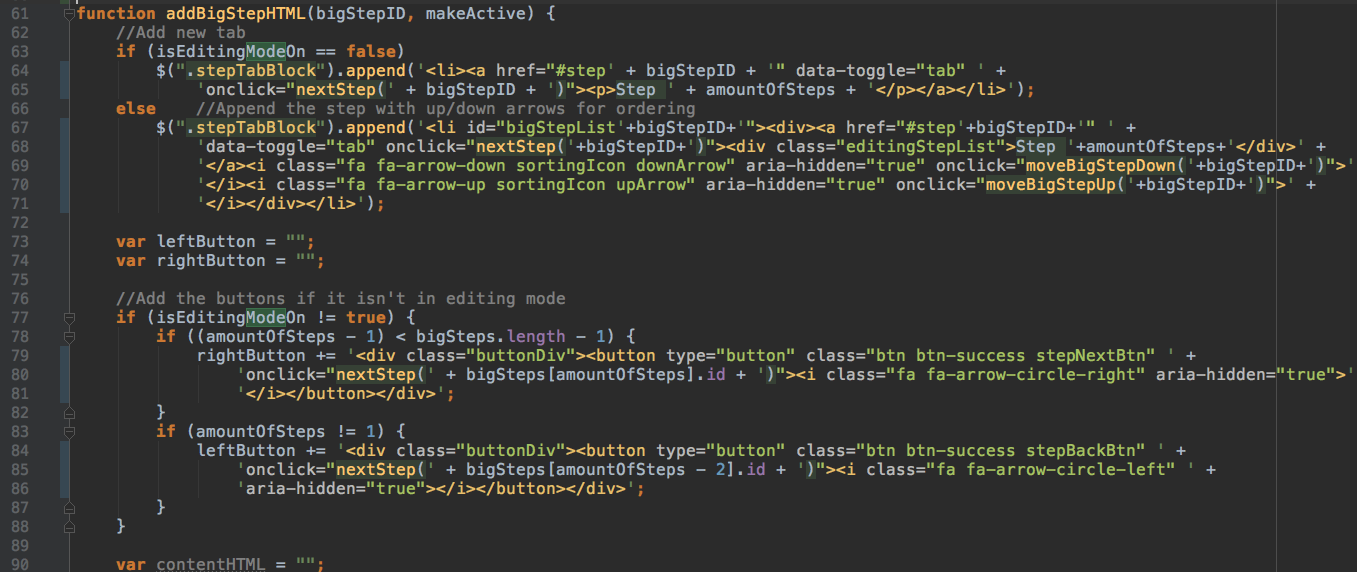
\includegraphics[width=1\linewidth]{images/stepsEdit&Present.png}
\caption{Show or Edit Steps Control Structure.}
\label{fig:edit_present_steps.}
\end{figure}	







Endpoints: 
/projects/index.php ==> display all projects / projects.js
/edit_project/{projectID}

projects/create_project/ ==> inserts a new project in db and takes the last inserted id + redirects to edit_project with the id:  header("Location: /smartfun/pages/projects/edit_project.php?projectId=lastInsertedProjectID");

/present_project/{projectID} / stars_ratings.js; projects_equipment.js; comments.js; addSteps.js
	




About MVC: 
- a function contained in views should not contain control structures or database requests 
- employing this paradigm allows very rapid integration of a completely new UI and fast responses to changes in UI requirements. (https://software.intel.com/en-us/blogs/2012/04/30/why-you-should-use-procedural-and-oop-in-every-application)
- disociating/isolating
- employing this paradigm allows very rapid integration of a completely new UI and fast responses to changes in UI requirements.




Endpoints: ?

\section{Security}












